\subsection{Análise exploratória}
\subsubsection{Quantidade de Órgãos Julgadores}

A Tabela \ref{tbl:tribunais_qtd_ojs} exibe a quantidade de órgãos julgadores por tribunal.

\begin{table}[ht]
\centering
\caption{Quantidade de órgãos julgadores por tribunal}
\begin{tabular}{cc|cc}
  \hline
  \multirow{2}{*}{\textbf{Tribunal}} & \multirow{2}{*}{\textbf{Estado}} &  \multicolumn{2}{c}{\textbf{Frequência}} \\
  \cline{3-4}
  &  & Absoluta & Relativa \\ 
 
   \hline
  TRT2 & SP & 319 & 14,23\% \\ 
  TRT1 & RJ & 222 & 9,91\% \\ 
  TRT15 & SP & 218 & 9,73\% \\ 
  TRT3 & MG & 210 & 9,37\% \\ 
  TRT4 & RS & 190 & 8,48\% \\ 
  TRT9 & PR & 140 & 6,25\% \\ 
  TRT5 & BA & 111 & 4,95\% \\ 
  TRT6 & PE &  97 & 4,33\% \\ 
  TRT12 & SC &  86 & 3,84\% \\ 
  TRT8 & AP e PA &  77 & 3,44\% \\ 
  TRT18 & GO &  64 & 2,86\% \\ 
  TRT7 & CE &  56 & 2,5\% \\ 
  TRT10 & DF e TO &  55 & 2,45\% \\ 
  TRT11 & AM e RR &  48 & 2,14\% \\ 
  TRT23 & MT &  45 & 2,01\% \\ 
  TRT13 & PB &  43 & 1,92\% \\ 
  TRT14 & AC e RO &  41 & 1,83\% \\ 
  TRT17 & ES &  41 & 1,83\% \\ 
  TRT24 & MS &  39 & 1,74\% \\ 
  TRT21 & RN &  35 & 1,56\% \\ 
  TRT19 & AL &  31 & 1,38\% \\ 
  TRT16 & MA &  26 & 1,16\% \\ 
  TRT22 & PI &  24 & 1,07\% \\ 
  TRT20 & SE &  23 & 1,03\% \\
  \hline
  \textbf{Total} & \textbf{Nacional} & 2.241 & 100\% \\ \hline
\end{tabular}
\label{tbl:tribunais_qtd_ojs}
\end{table}

Dos tribunais trabalhistas, o que conta com maior representação em quantidade de órgãos julgadores é o TRT2, com pouco mais de 13\% do total nacional. Dois dos tribunais trabalhistas com mais órgãos julgadores são pertencentes ao estado de São Paulo, correspondendo, juntos, a quase 25\% do total nacional. O estado de São Paulo é, também, a única unidade federativa com dois tribunais da Justiça do Trabalho.

Há quatro tribunais da Justiça do Trabalho que possuem jurisdição em mais de uma Unidade da Federação (UF): TRT8, TRT10, TRT11 e TRT14. Todos esses se restringem a operar em duas UFs cada.

A diferença entre os tribunais para cada ranking decresce de forma suave, sem nenhum grande salto entre um colocado e seu posterior ou anterior. O ramo trabalhista conta com um total de 2.241 órgãos julgadores.


\subsubsection{Distribuição dos tempos}
\begin{figure}[H]
    \centering
    \caption{Distribuição dos tempos até a baixa}
    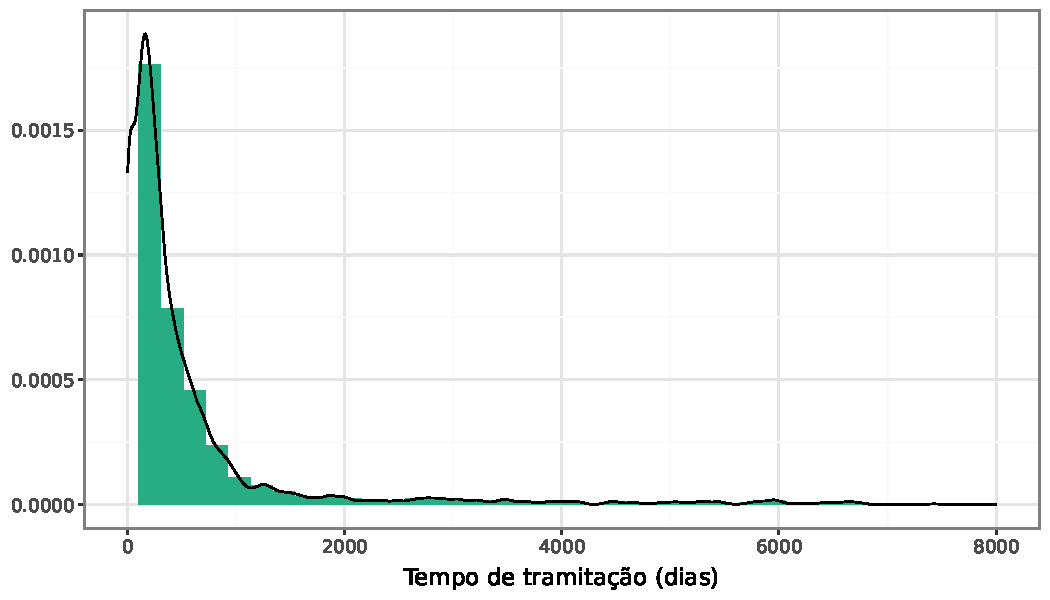
\includegraphics[scale=.85]{imagens/dist_tempo.pdf}
\end{figure}

Dado que se trata do tempo entre uma situação e outra posterior à primeira, todos os valores observados são não-negativos. A maior parte dos processos leva até 2.000 dias para receber baixa. 

A distribuição dos tempos é assimétrica à direita, quase que rigorosamente decrescente. Esse comportamento, por sua vez, não se assemelha ao comportamento de uma distribuição normal, que é simétrica e possui valores negativos com probabilidade não-nula.

Devido à quantidade excessiva de observações, foram feitas 10 amostras aleatórias simples de tamanho 500 sem reposição, e aplicado, para cada, o teste de normalidade de Shapiro-Wilk sob nível de significância de 5\%. As hipóteses foram:

$\begin{cases}
H_{0}: \mbox{O tempo até a baixa segue distribuição Normal.} \\
H_{1}: \mbox{O tempo até a baixa não segue distribuição Normal.}  \\
\end{cases}
$\\

\begin{table}[H]
\centering
\caption{Teste de normalidade de Shapiro-Wilk para amostras do tempo até a baixa}
\begin{tabular}{cccc}
\hline
\textbf{Teste} & \textbf{Variáveis} & \textbf{P-valor máximo} & \textbf{Decisão do teste} \\ \hline
Shapiro-Wilk & Tempo até a baixa & $\approx 0$   & Rejeita $H_0$  \\ \hline  
\end{tabular}
\label{teste:normalidade_tempo}
\end{table}

A Tabela \ref{teste:normalidade_tempo} mostra que mesmo o maior p-valor obtido ainda foi próximo de zero. Para todos os testes, a hipótese de normalidade do tempo até a baixa de um processo foi rejeitada, apresentando, assim, evidências de que sua distribuição não é normal.


\subsubsection{Formato dos processos}\label{sec:formato}
O Conselho Nacional de Justiça instituiu o Processo Judicial Eletrônico (PJe) como forma de tornar o Poder Judiciário mais célere \cite{pje}. A comparação entre os formatos de processos é relevante, não só pela predição do tempo até a baixa, mas também para observar se os resultados da instituição do PJe correspondem aos esperados pelas instituições de justiça.

Espera-se que a quantidade de casos novos físicos diminua progressivamente ao longo do tempo, até se aproximar de zero. A Figura \ref{fig:pct_fisicos_tempo} mostra essa evolução de janeiro 2021 até janeiro de 2024.

\begin{figure}[H]
    \centering
    \caption{Evolução da frequência relativa de casos novos físicos ao longo do tempo}
    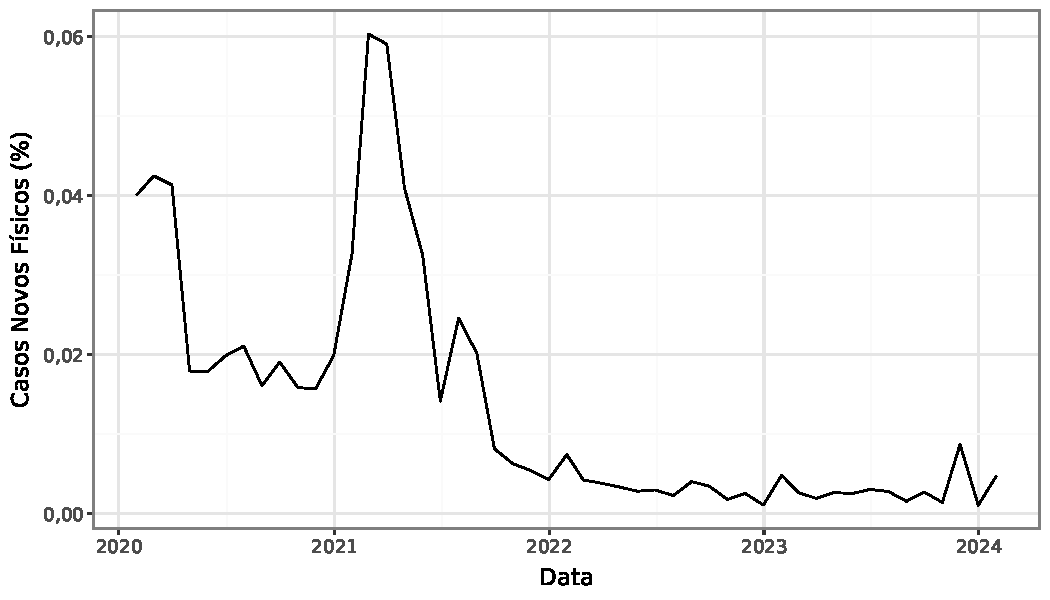
\includegraphics[scale=.87]{imagens/pct_fisicos_tempo.pdf}
    \label{fig:pct_fisicos_tempo}
\end{figure}

A Figura \ref{fig:pct_fisicos_tempo} mostra uma tendência geral de queda. A frequência relativa de casos novos físicos já era de apenas 0,06\% em 2021, e seguiu em queda, chegando a valores muito próximos de zero no começo de 2024.

A Figura \ref{fig:pct_fisicos_tramitando_tempo} mostra a evolução da frequência de processos físicos pendentes tramitando ao longo dos últimos anos.

\begin{figure}[H]
    \centering
    \caption{Evolução da frequência relativa de processos pendentes tramitando em formato físico ao longo do tempo}
    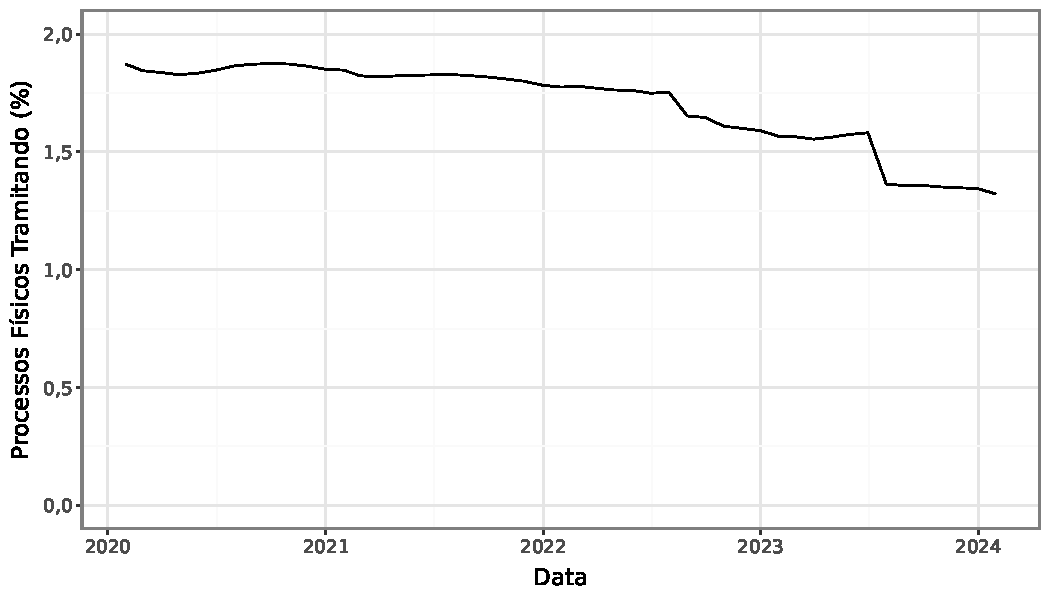
\includegraphics[scale=.85]{imagens/pct_fisicos_tramitando_tempo.pdf}
    \label{fig:pct_fisicos_tramitando_tempo}
\end{figure}

A frequência de processos físicos tramitando permanece relativamente estável e acima de 1\%, apesar de o número de casos novos físicos cair em ritmo acelerado. A discrepância mostra que a maior parte destes processos eletrônicos pendentes não foi iniciada durante o período, sugerindo que os processos com formato físico podem chegar a durar vários anos. A baixa frequência de processos físicos em tramitação também indica que essa variável se trata de um fenômeno raro, em especial durante o período.

A Figura \ref{fig:formato_tempo} mostra a distribuição dos tempos entre o início do processo e a data de referência para cada um dos formatos, onde há processos ainda ativos. Foram omitidos quaisquer processos para os quais o formato era indisponível.

\begin{figure}[H]
    \centering
    \caption{Distribuição dos tempos de tramitação dos processos para cada formato em processos ainda ativos}
    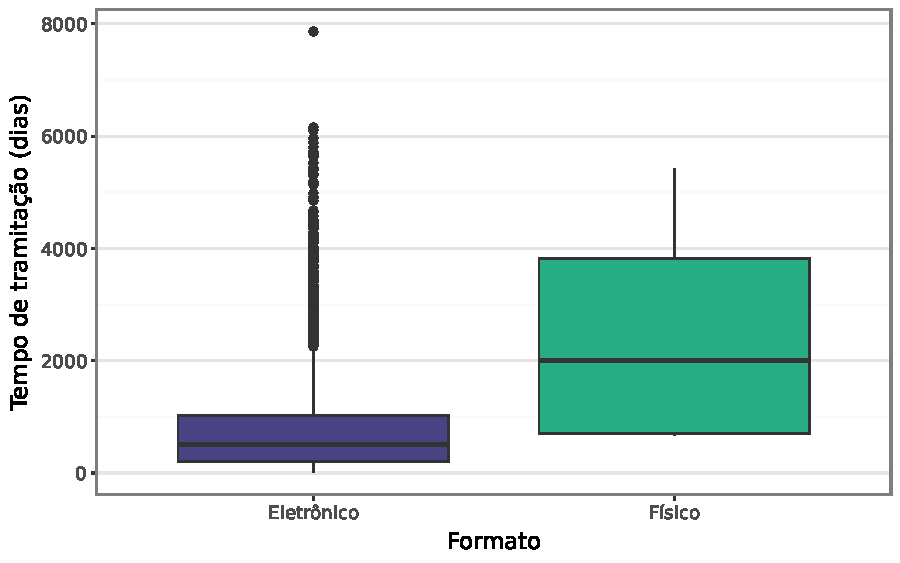
\includegraphics[scale=.93]{imagens/formato_tempo.pdf}
    \label{fig:formato_tempo}
\end{figure}

A Figura \ref{fig:formato_tempo} mostra uma discrepância grande de magnitude entre os tempos de processos físicos e eletrônicos. Cerca de 50\% dos processos físicos tramitando possuem tempo de tramitação próxima ou maior que seis anos.

Além da clara diferença no tempo entre os formatos, há uma variabilidade muito menor dos processos eletrônicos em relação aos processos físicos, que indica que os processos eletrônicos podem ter predições mais precisas.

A diferença sugere que o PJe, de fato, tornou os processos mais céleres, conforme as expectativas do Conselho Nacional de Justiça.


\subsubsection{Graus de jurisdição\label{sec:graus}}
O Poder Judiciário é hierarquizado por três graus de jurisdição: o Primeiro Grau, o Segundo Grau e os Tribunais Superiores. O Primeiro Grau, por sua vez, é também o grau com maior carga processual, fato que motivou a instauração da Política Nacional de Priorização do Primeiro Grau, equilibrando orçamento e pessoal entre os graus segundo suas demandas \cite{justicaemnumeros}.

A Figura \ref{fig:grau_tempo} mostra a distribuição dos tempos até a baixa para o primeiro e segundo graus de jurisdição. Foi feito um corte no eixo Y para evitar que os outliers prejudiquem a visualização.

\begin{figure}[H]
    \centering
    \caption{Distribuição dos tempos até a baixa dos processos para o primeiro e o segundo graus de jurisdição}
    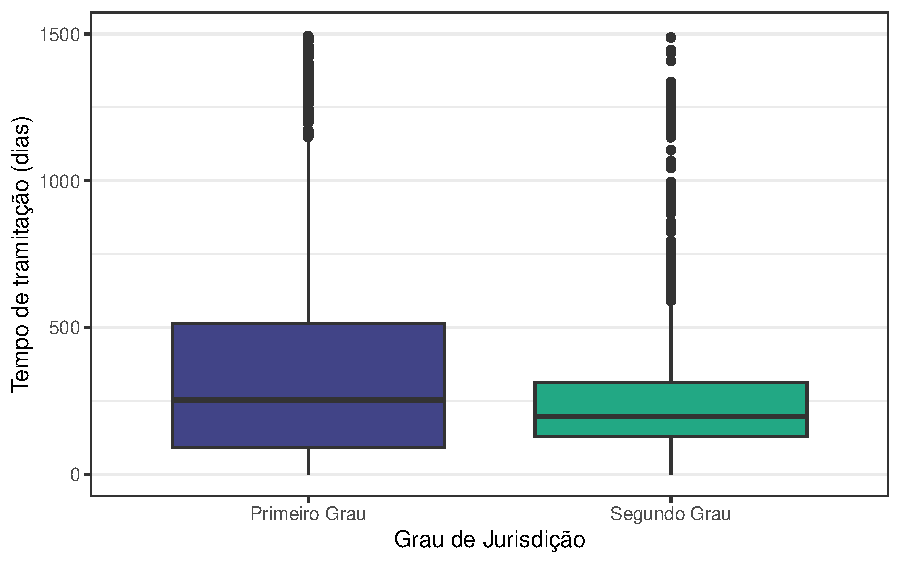
\includegraphics[scale=1]{imagens/grau_tempo.pdf}
    \label{fig:grau_tempo}
\end{figure}

Os tempos até a baixa de um processo são consistentemente menores para o segundo grau, quando comparados com o primeiro. De fato, a discrepância que o Relatório Justiça em Números aponta entre o Primeiro Grau e os outros graus de jurisdição ainda é refletida nos indicadores, tornando o grau uma variável candidata relevante para a predição dos tempos.

\subsubsection{Recursos\label{sec:recursos}}
A primeira decisão judicial sobre um processo é tomada em sua competência originária. Em caso de impugnação de alguma das partes envolvidas no processo, é aberto um recurso para revisar a decisão. O eixo Y foi cortado para evitar prejuízo à visualização devido aos outliers.

\begin{figure}[H]
    \centering
    \caption{Distribuição dos tempos até a baixa dos processos originários e recursais}
   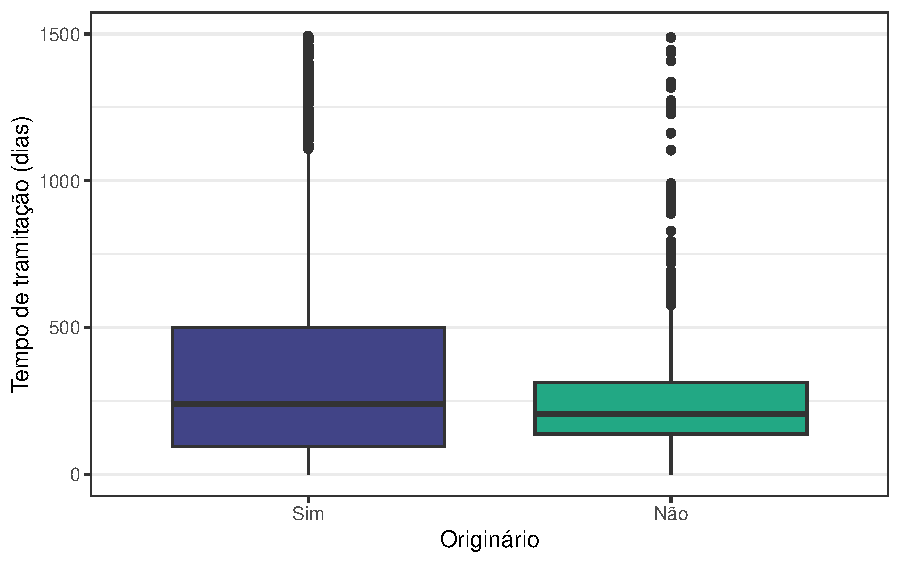
\includegraphics[scale=1]{imagens/originario.pdf}
    \label{fig:originario}
\end{figure}

A Figura \ref{fig:originario} mostra uma diferença de dispersão e de magnitude, onde não só os recursos são mais céleres, como também são concentrados em um intervalo menor.

Ainda, o comportamento dos processos originários e recursais é muito parecido com o comportamento dos processos de primeiro e segundo grau, o que pode indicar associação entre as variáveis. Essa possível associação será discutida na Seção \ref{sec:associacoes_vars}.


\subsubsection{Associação entre as variáveis qualitativas\label{sec:associacoes_vars}}
Foi observada uma semelhança entre os tempos até a baixa nos gráficos da Seção \ref{sec:recursos} e a Seção \ref{sec:graus}.  A Tabela \ref{tbl:originario_grau} investiga as frequências cruzadas de ocorrências de cada grau e nível de recurso.

\begin{table}[H]
\centering
\caption{Frequência de processos pendentes cruzada por grau e recursos}
\begin{tabular}{c|cc|c}
\hline
\multirow{2}{*}{\textbf{Grau}} & \multicolumn{2}{c|}{\textbf{Originário}} & \multirow{2}{*}{\textbf{Total}} \\ 
\cline{2-3}
 & Sim & Não \\ 
  \hline
1º & 5.284.459 &   0  & 5.284.459 \\ 
2º & 113.080 & 670.461 & 783.541 \\ 
   \hline
  Total & 5.397.539 & 670.461 & 6.068.000 \\ 
\hline
\end{tabular}
\label{tbl:originario_grau}
\end{table}

Olhando através dos níveis de recurso, é perceptível que a maior parte das ocorrências originários está compreendida em primeiro grau, bem como a maior parte das ocorrências não-originárias está compreendida em segundo grau. Dentre os processos de segundo grau, há cerca de seis vezes mais processos recursais do que processos originários, e nenhum dos processos recursais observados no período pertence ao primeiro grau.

Visando investigar possíveis outras associações, serão aplicados testes de associação entre as variáveis qualitativas. A Tabela \ref{tbl:assoc_categoricas} exibe o resultado dos testes bivariados de independência para procedimento, grau, originário e formato.

O teste exato de Fisher foi aplicado em todas as tabelas 2x2. Para as tabelas com dimensão maior, foi utilizado o teste Qui-Quadrado de independência.

\begin{table}[H]
\centering
\caption{Testes para Independência entre Variáveis Categóricas}
\begin{tabular}{cccc}
\hline
\textbf{Teste} & \textbf{Variáveis} & \textbf{P-valor} & \textbf{Decisão do teste} \\ \hline
Qui-Quadrado & Grau x Procedimento & $\approx 0$   & Rejeita $H_0$  \\
Qui-Quadrado & Procedimento x Originário & $\approx 0$   & Rejeita $H_0$  \\
Qui-Quadrado & Procedimento x Formato & 0,628   & Não rejeita $H_0$  \\
Exato de Fisher & Formato x Grau & 0,307 & Não rejeita $H_0$  \\
Exato de Fisher & Formato x Originário & 0,585 & Não rejeita $H_0$  \\
Exato de Fisher & Grau x Originário & $\approx 0$   & Rejeita $H_0$  \\ \hline 
\end{tabular}
\label{tbl:assoc_categoricas}
\end{table}

Não há evidências de que a informação sobre o procedimento esteja associada ao processo ser físico ou eletrônico. Apesar disso, a hipótese de independência foi rejeitada entre procedimento e grau, bem como em procedimento e originário. O teste também confirma o que era apontado pela Tabela \ref{tbl:originario_grau}, mostrando evidências de associação entre grau e originário. Para as outras variáveis, não foram encontradas evidências significativas de associação.


\subsubsection{Procedimentos}\label{sec:procedimento}
\begin{figure}[H]
    \centering
    \caption{Distribuição dos tempos até a baixa dos processos segundo o procedimento}
    \label{fig:procedimentos_tempo}
    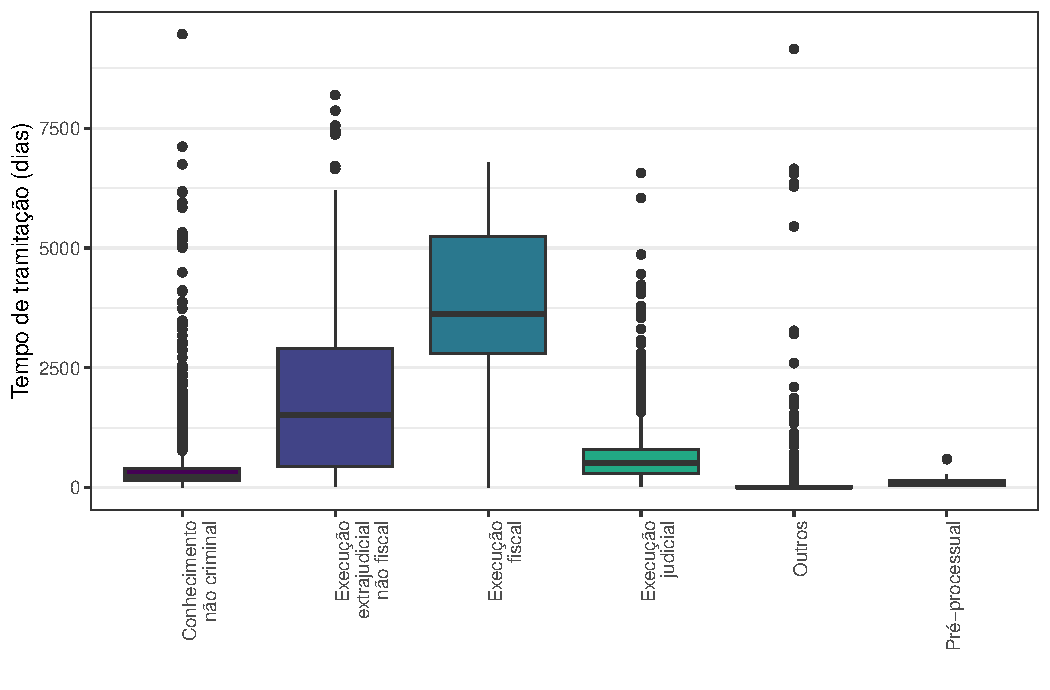
\includegraphics[scale=.9]{imagens/procedimento_tempo.pdf}
\end{figure}

É notável que os procedimentos de conhecimento tendem a apresentar tempos drasticamente menores que os procedimentos de execução. Os pré-processuais e outros, que apresentaram as menores tendências de tempo entre todos os procedimentos observados.

Além da diferença quantitativa entre as execuções, cada execução apresentou um padrão diferente de dispersão. A execução judicial foi a que menos variou entre os três procedimentos de execução. A execução fiscal não apresentou nenhum outlier e teve o maior valor mediano dentre todos os procedimentos, além de apresentar comportamento assimétrico.

\subsubsection{Indicadores quantitativos}
Dos 26 indicadores presentes na Tabela Fato, alguns são correlacionados com outras métricas de forma direta \cite{painelestatistica}. Estão entre eles:
\begin{itemize}
    \item Total de processos Conclusos para o Magistrado a mais de 50 dias: Está correlacionado com o indicador de Conclusos para o Magistrado.
    \item Processos sem tramitação há mais de 50 dias: Está correlacionado ao indicador de Tramitando.
    \item 5\% mais antigos em tramitação: Corresponde a 5\% dos processos no indicador de Tramitando.
    \item Tramitando (ou Pendentes líquidos): Agrega todos os processos que não receberam Baixa, Suspensão ou Sobrestamento.
    \item Pendentes: Agregam todos os processos que não receberam Baixa, incluindo Tramitando, Suspensos e Sobrestados.
    \item Conclusos: Agrega Conclusos para Julgamento, para Despacho, para Admissibilidade recursal, para Decisão, sem especificação e outros.
    \item Audiências: Agrega Audiências Conciliatórias e Não Conciliatórias.
\end{itemize}


Em decorrência das correlações, serão escolhidas as métricas que, sozinhas, agregam a maior quantidade de outros indicadores. A exceção a essa regra será o indicador da situação Tramitando, bem como Suspensos e Sobrestados (que, juntos, constituiriam os Pendentes). Assim sendo, os indicadores são: Tramitando, Suspensos e Sobrestados, Conclusos, Julgamentos, Despachos, Decisões, Audiências, Total de liminares deferidas, Total de liminares indeferidas, Casos Novos de Recurso Interno, Recurso Interno Pendente e Recurso Interno Julgado. A Figura \ref{fig:inds_qtd} mostra a quantidade de ocorrências de cada um dos indicadores selecionados. Apesar de o indicador Pendentes não ter sido incluído, a informação completa dele está incluída, uma vez que os Pendentes são a soma de Tramitando, Suspensos e Sobrestados. Os processos Suspensos e Sobrestados, por simplicidade, serão referidos no documento apenas como “Suspensos”.

\begin{figure}[H]
    \centering
    \caption{Quantidade de ocorrências em cada métrica}
    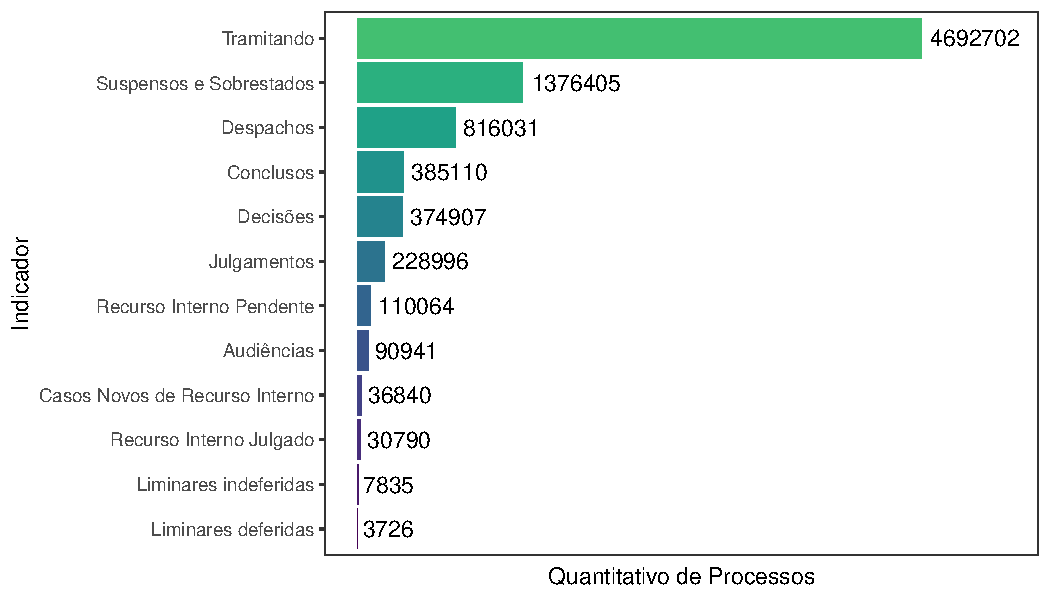
\includegraphics[scale=.9]{imagens/inds_qtd.pdf}
    \label{fig:inds_qtd}
\end{figure}

A quantidade de processos Tramitando é a predominante dentre todos os indicadores exibidos. Nos dois indicadores mais frequentes, há um salto entre o primeiro e o segundo, onde o quantitativo de processos Tramitando é mais de três vezes superior ao número de Suspensos.

Os demais indicadores decaem com poucos saltos, onde os indicadores com menor representação são os de liminares indeferidas e liminares deferidas. Estes, por sua vez, têm uma quantidade de processos pouco maior do que a quantidade de órgãos julgadores. Nota-se que a quantidade de liminares deferidas tem uma média de pouco mais de 1,5 liminares para cada órgão julgador.


A Figura \ref{fig:corr_matrix} investiga possíveis correlações das variáveis explicativas entre elas. 
\begin{figure}[H]
    \centering
    \caption{Matriz de correlações entre as variáveis explicativas}
    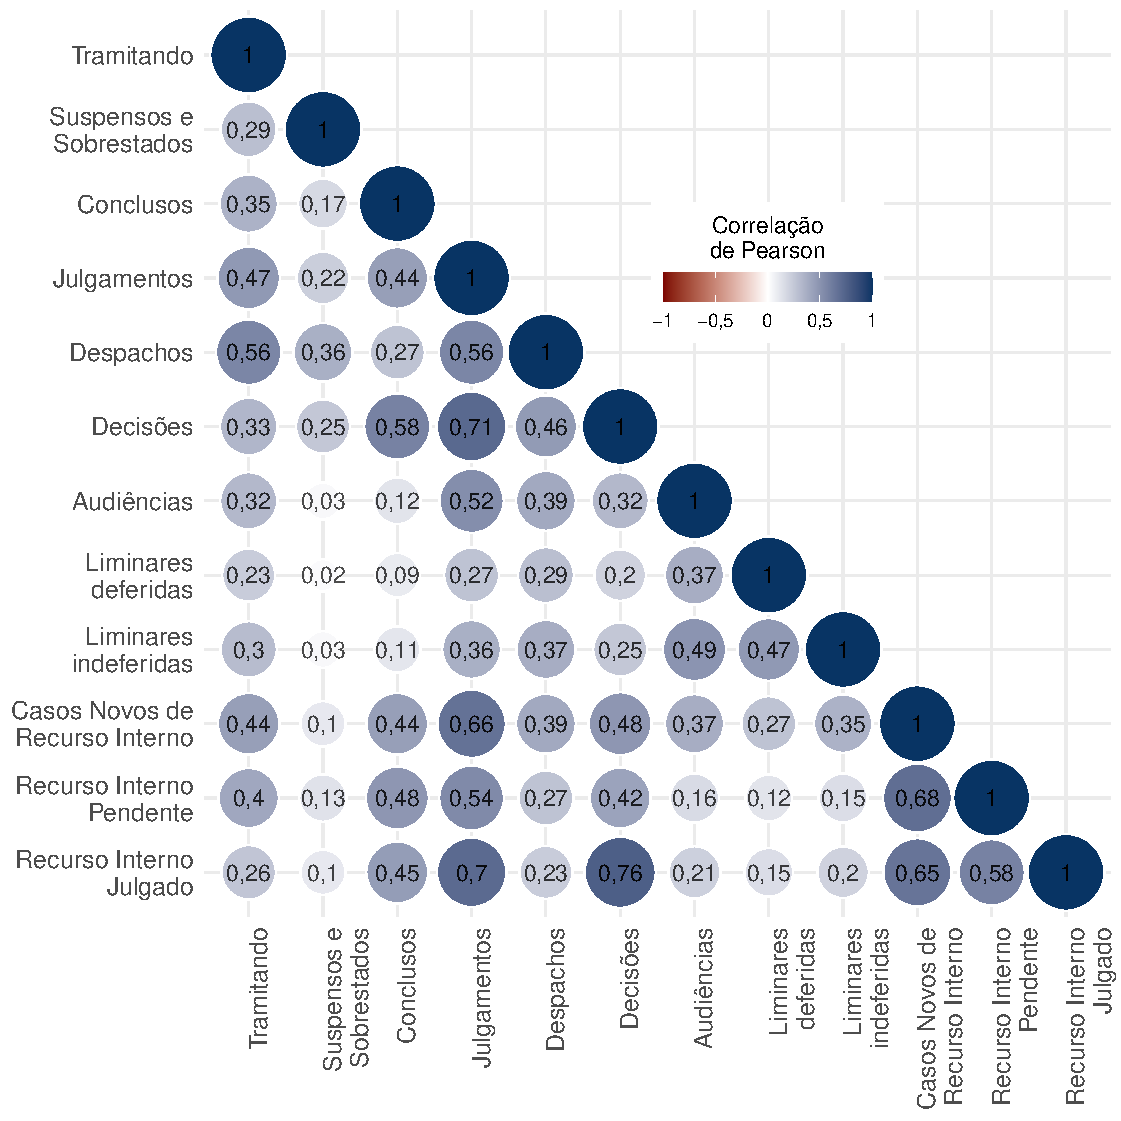
\includegraphics[scale=0.8]{imagens/corrplot.pdf}
    \label{fig:corr_matrix}
\end{figure}

Não houve nenhuma correlação negativa dentre todas as observadas na matriz, embora haja diversas correlações muito próximas de zero.

Os Casos Novos de Recurso Interno, Recurso Interno Pendente e Recurso Interno Julgado, apesar de não conterem um ao outro (como é o caso de outras variáveis supracitadas), não só se correlacionam pelo fato de tratarem de fenômenos relacionados aos recursos internos, como apresentam uma correlação de moderada a forte (aproximadamente de 0,6), com intensidade próxima para todos eles. O indicador Recurso Interno Julgado apresenta uma correlação ainda mais forte com as variáveis Decisões e Julgamentos, que configuraram, também, as maiores correlações observadas na matriz.

As Decisões e Julgamentos, por sua vez, também estão correlacionadas entre elas com intensidade próxima à de Recursos Internos Julgados. Houve uma intensidade moderada entre os dois indicadores e o quantitativo de Conclusos.

Os dois indicadores de Liminares (deferidas e indeferidas), Audiências, Despachos, Conclusos e Suspensos, não mostraram correlações fortes com nenhum indicador. Os maiores valores registrados para a correlação das liminares indeferidas foram 0,49 e 0,47, com, respectivamente, as variáveis de Audiências e Liminares deferidas. Os outros indicadores citados, eventualmente, apresentaram correlações moderadas entre eles, onde os Conclusos tiveram a maior de suas correlações com as Decisões e os Despachos tiveram suas maiores correlações com Tramitando e Julgamentos.

O indicador Tramitando, mesmo com maior representatividade dentre todos os indicadores, não apresentou correlação forte com nenhum deles, tendo variado entre fraca e moderada.

Os Suspensos foram os casos que apresentaram menores correlações com todos os indicadores, com valores maiores que 0,3 apenas quando correlacionados com os Despachos.

\subsubsection{Tempo até a baixa por indicador}

A Figura \ref{fig:cross_charts} mostra gráficos de dispersão de cada variável explicativa contra o tempo até a baixa dos processos. A reta azul indica a reta de regressão quantílica para a mediana, enquanto a reta verde indica a reta de regressão gaussiana para a média.

\begin{figure}[H]
    \centering
    \caption{Gráficos de dispersão entre as variáveis explicativas e o tempo até a baixa com retas de regressão quantílica (mediana, em azul) e regressão gaussiana (média, em verde)}
    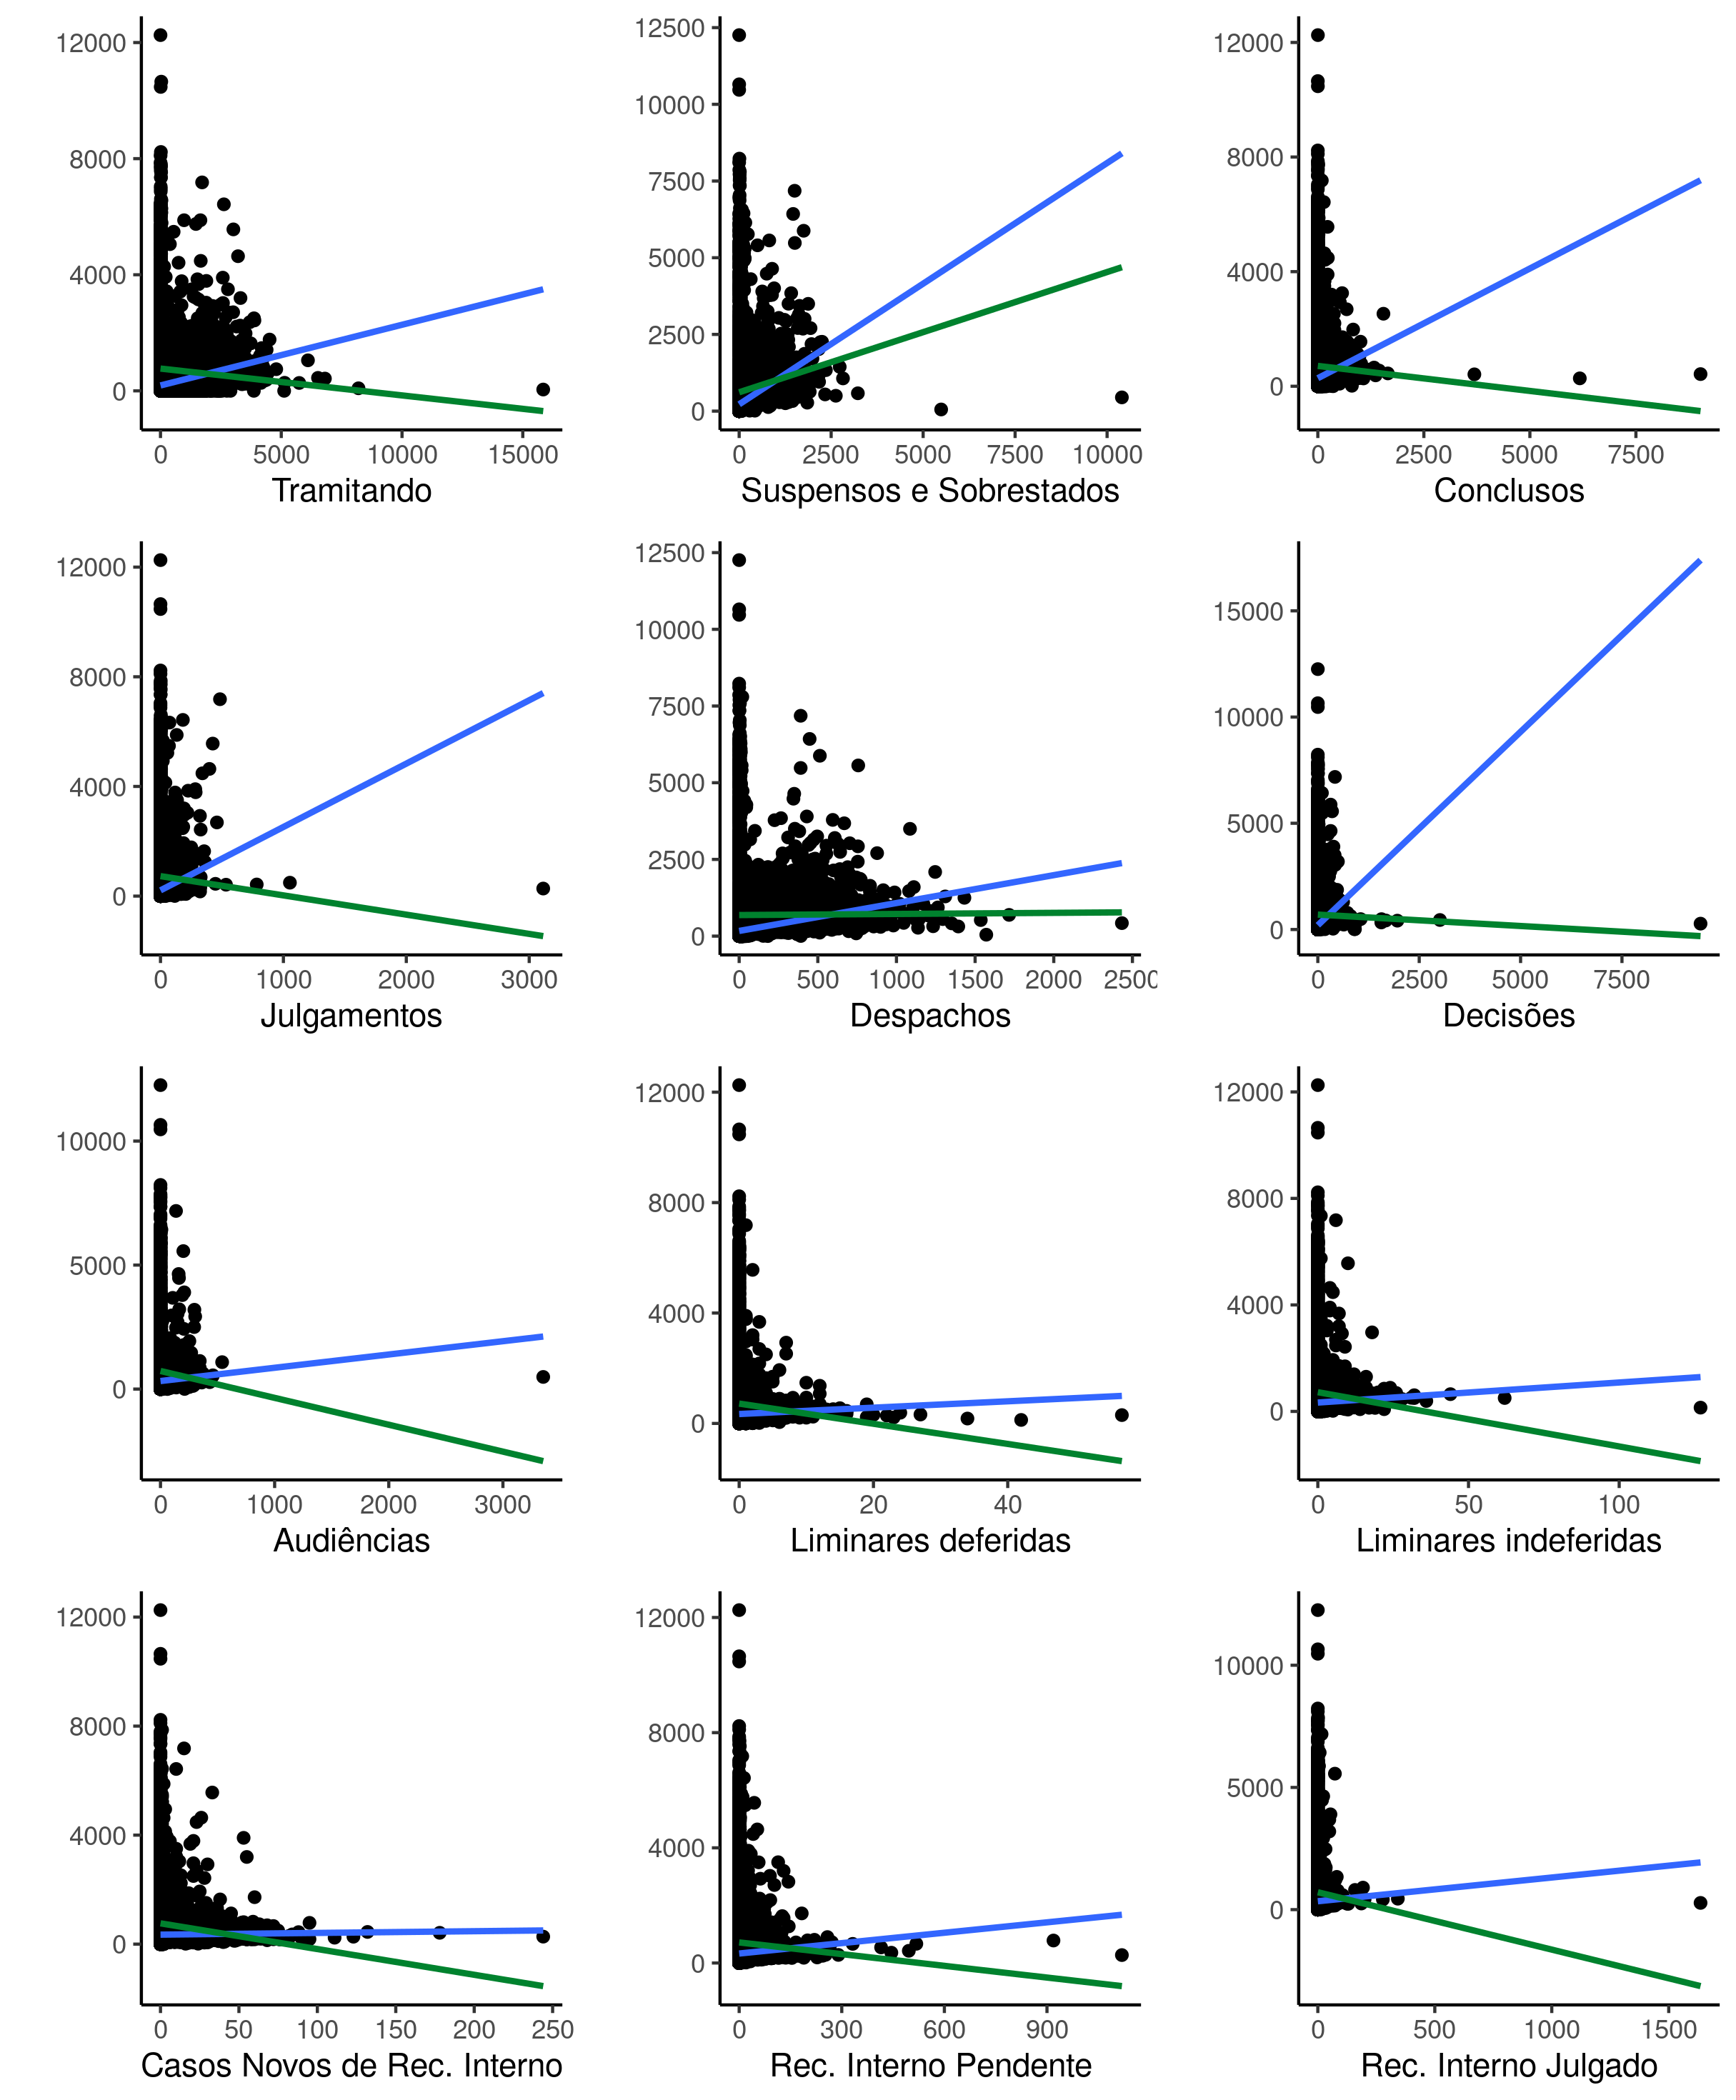
\includegraphics[scale=.745]{imagens/cross_charts.png}
    \label{fig:cross_charts}
\end{figure}

Na visualização bidimensional, não há, segundo os modelos quantílicos, qualquer indicativo de tendência de decrescimento para o tempo mediano de tramitação dos processos conforme o crescimento de um indicador, de modo que esperam-se coeficientes positivos em quaisquer lugares onde eles sejam não-nulos. Apesar disso, vários dos modelos de regressão por mínimos quadrados apresentaram retas decrescentes, eventualmente podendo levar a valores inferiores a zero, sendo eles: Conclusos, Julgamentos, Decisões, Audiências, Liminares deferidas, Liminares indeferidas, Casos Novos de Rec. Interno, Rec. Interno Pendente e Rec. Interno Julgado, de modo que não só a reta mediana e a reta média não coincidem, como se contradizem. Nota-se que a regressão gaussiana é mais suscetível à influência de outliers do que a regressão quantílica.

Apesar de, graficamente, os Casos Novos de Recurso Interno aparentarem ter uma menor inclinação, as inclinações estão prejudicadas não só pela escala do eixo X e Y serem diferentes, como também pela presença de outliers nas variáveis explicativas.

Em todos os indicadores, existe uma concentração grande das observações em torno do valores onde a variável explicativa é próxima de zero. Fica notável a presença de vários órgãos julgadores que, apesar de relatarem poucos processos tramitando, levam um tempo significativamente grande para dar baixa nos processos que existem. A Tabela \ref{tbl:caracteristicas_pendentes_tempo_longo} exibe características das varas com menos de 120 processos pedentes e tempo até a baixa maior que 1.000 dias. 


\begin{table}[ht]
\centering
\caption{Características das varas com menos de 120 processos tramitando e mais de 1.000 dias de tempo até a baixa}
\begin{tabular}{llll|cc}
  \hline
  \textbf{Formato} & \textbf{Grau} & \textbf{Originário} & \textbf{Procedimento} & \textbf{Ocorrências} & \textbf{Tempo} \\ 
  \hline
  Eletrônico & 1º & Sim & Execução fiscal & 267 & 4299 \\ 
  Eletrônico & 1º & Sim & Execução extrajudicial não fiscal &  69 & 3978 \\ 
  Eletrônico & 2º & Não & Conhecimento não criminal &  25 & 1830 \\ 
  Eletrônico & 2º & Sim & Conhecimento não criminal &  22 & 1411 \\ 
  Eletrônico & 1º & Sim & Execução judicial &   3 & 3220 \\ 
  Eletrônico & 1º & Sim & Conhecimento não criminal &   1 & 3295 \\ 
  Físico & 1º & Sim & Conhecimento não criminal &   1 & 9466 \\ 
  Físico & 1º & Sim & Execução judicial &   1 & 3085 \\ 
   \hline
\end{tabular}
\label{tbl:caracteristicas_pendentes_tempo_longo}
\end{table}


A Tabela \ref{tbl:caracteristicas_pendentes_tempo_longo} mostra que, das varas com menos de 120 processos tramitando e com tempo até a baixa acima de 1.000 dias, 336 (86,37\%) delas estão entre os processos eletrônicos de primeiro grau, originários, com procedimento de execução (fiscal e extrajudicial não fiscal). Esse comportamento está dentro do  esperado, uma vez que, como já observado na Figura \ref{fig:procedimentos_tempo}, os dois procedimentos citados possuem tanto maiores tempos até a baixa quanto maior dispersão nesses tempos, bem como os processos originários e de primeiro grau.

Poucas ocorrências relatavam processos físicos, mas, das que relatavam, há uma vara com processos físicos cujo tempo até a baixa foi de quase 10.000 dias, que foi o maior valor registrado na tabela. Essa vara tinha procedimento de conhecimento não criminal, que foi o único procedimento de conhecimento relatado nos grupos observados, e também o procedimento de conhecimento com maiores tempos até a baixa (Figura \ref{fig:procedimentos_tempo}).

A Figura \ref{fig:cross_charts_without_outliers} exibe os mesmos diagramas de dispersão, com a remoção dos outliers das variáveis explicativas e remoção das quatro categorias da Tabela \ref{tbl:caracteristicas_pendentes_tempo_longo} que apresentaram os maiores tempos até a baixa. A reta azul indica a reta de regressão quantílica para a mediana, enquanto a reta verde indica a reta de regressão gaussiana para a média.

\begin{figure}[H]
    \centering
    
    \caption{Gráficos de dispersão entre as variáveis explicativas e o tempo até a baixa com retas de regressão quantílica (mediana, em azul) e regressão gaussiana (média, em verde), com remoção de outliers}
    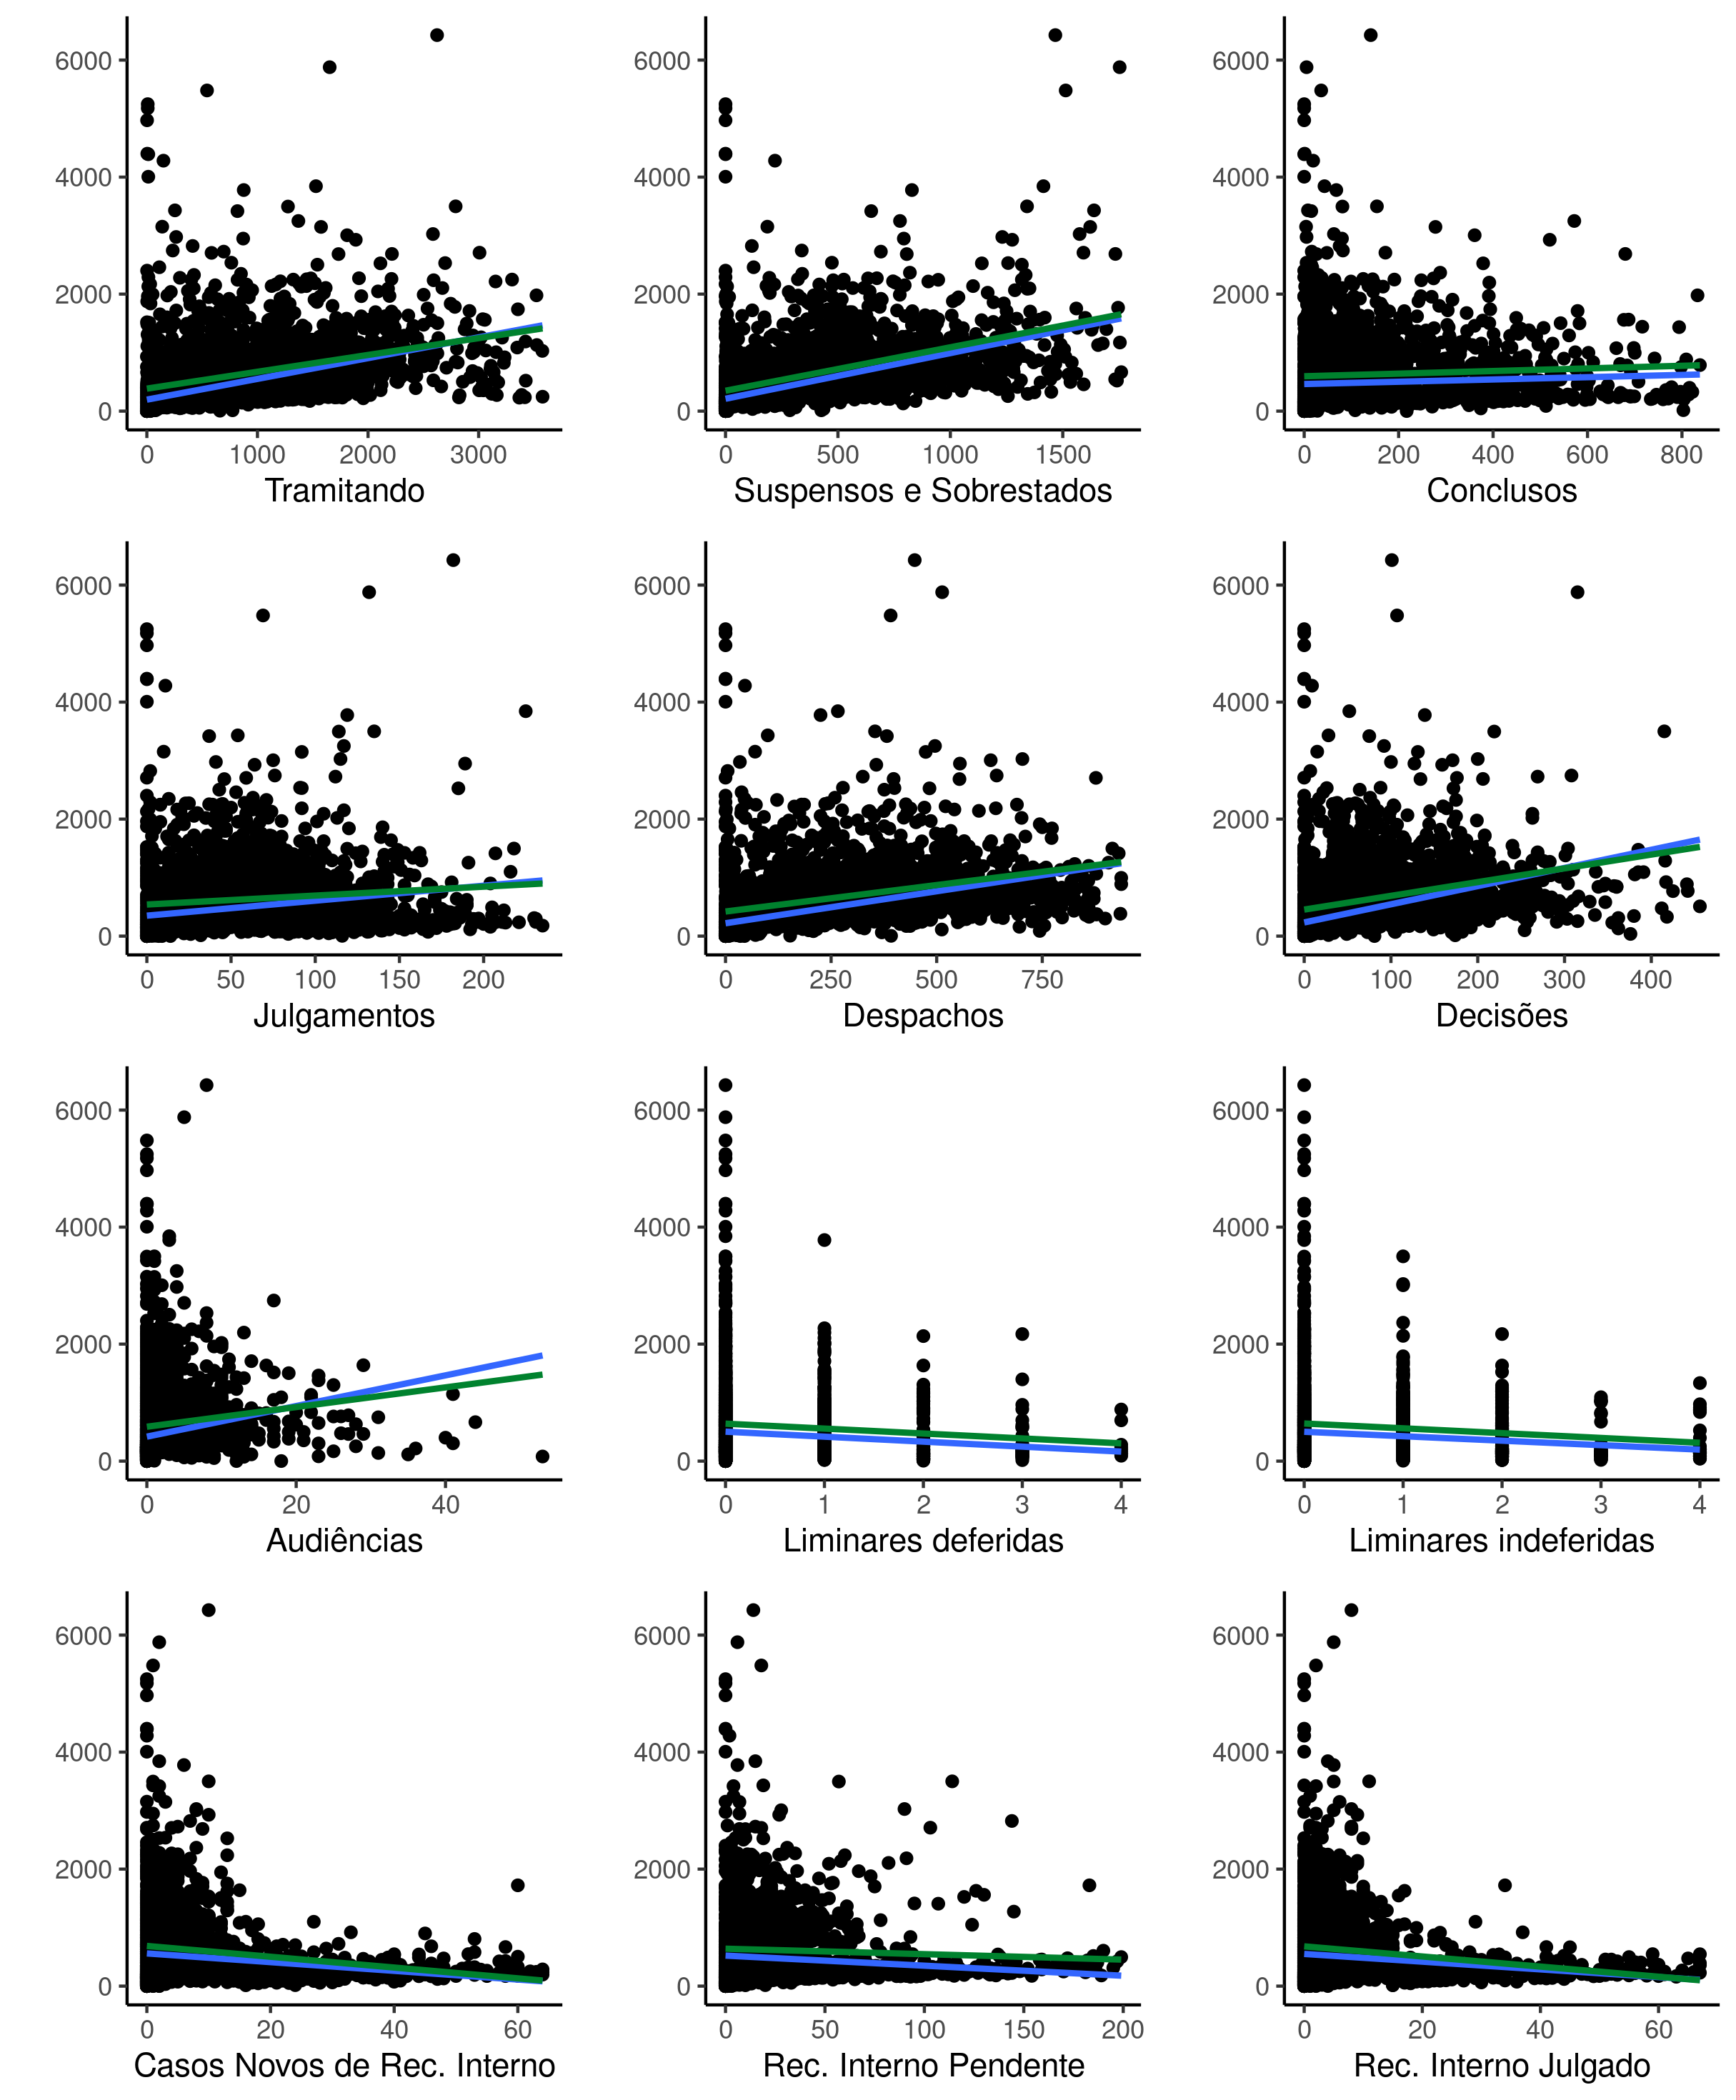
\includegraphics[scale=.74]{imagens/cross_charts_without_outliers.png}
    \label{fig:cross_charts_without_outliers}
\end{figure}

Com a remoção das categorias supracitadas, quase todas as contradições de tendência entre as médias e as medianas sumiram para todas as variáveis explicativas observadas. Ainda, até mesmo a proximidade das retas aumentou, fornecendo valores, visualmente, muito próximos entre elas.

As retas medianas permaneceram estritamente crescentes. Já as retas médias ainda apresentaram um comportamento que aparenta estar entre o decrescente e o constante para as Audiências, Liminares deferidas, Liminares indeferidas e Casos Novos de Rec. Interno.

As audiências, liminares e recursos internos ainda apresentam dispersão maior dos tempos até a baixa para valores pequenos das variáveis explicativas, bem como tempos propriamente ditos consideravelmente maiores onde os valores das variáveis explicativas eram próximos de zero. O comportamento delas é não-linear, e elas possuem uma amplitude muito pequena quando comparadas às outras seis variáveis.





\newpage
\subsection{Modelos}

Para a construção dos modelos, os dados foram filtrados para conter apenas o retrato do mês de janeiro. Foram utilizadas todas as observações do filtro. A seleção de variáveis foi feita utilizando \textit{stepwise} bidirecional e o AIC como critério de seleção. Uma vez selecionado um modelo com o menor AIC, será feita uma outra seleção de variáveis utilizando \textit{stepwise} pelo teste de significância dos parâmetros, removendo a variável com o maior p-valor e ajustando um modelo sem ela, repetindo o processo até que todas as variáveis tenham um p-valor menor que 0,1.

\subsubsection{Modelos para a mediana}
\label{modelos_mediana}
O Modelo \ref{tab:candidate1_0,5} mostra o resultado do ajuste considerando todas as covariáveis de forma independente, sem quaisquer interações ou componentes não-lineares.

\begin{modelo}[H]
\centering
\caption{Regressão quantílica ($\tau$ = 0,5)} 
\label{tab:candidate1_0,5}
\begin{tabular}{c|cc|c}
  \hline
\textbf{Variável} & \textbf{Coeficiente} & \textbf{Erro Padrão} & \textbf{P-valor} \\ 
  \hline
  Intercepto & 7,1 meses & 18 & \approx 0 \\ 
  Procedimento - Pré-processual & -3,6 meses & 36 & 0,002 \\ 
  Procedimento - Outros & -1 mês & 12 & 0,012 \\ 
  Grau & -2,1 meses & 18 & \approx 0 \\ 
  Tramitando & 2h29min & 0,007 & \approx 0 \\ 
  Suspensos & 3h53min & 0,024 & \approx 0 \\ 
  Despachos & 5h12min & 0,041 & \approx 0 \\ 
  Decisões & -7h56min & 0,097 & 0,009 \\ 
  Conclusos & 4h4min & 0,076 & 0,026 \\
   \hline
\end{tabular}
\end{modelo}

No que se refere às variáveis qualitativas, a variável "Formato" não se mostrou relevante, contrariando as expectativas geradas pela Seção \ref{sec:formato}, na qual a variável foi avaliada incondicionalmente e de forma exploratória. Apesar disso, tanto as expectativas da Seção \ref{sec:graus} quanto da Seção \ref{sec:procedimento} foram confirmadas, dado que o Grau e alguns procedimentos foram considerados relevantes. É notável que os procedimentos resultantes estão entre os procedimentos que apresentaram o menor tempo, e apresentaram coeficientes negativos, portanto.

Todas as variáveis quantitativas apresentaram evidências estatisticamente significativas para rejeição da hipótese de ausência de regressão, conforme o método de seleção induz. A variável "Decisões" foi a única variável quantitativa cujo coeficiente foi negativo.

Quase todas as covariáveis resultantes apresentam uma correlação fraca entre elas, como se pode observar retornando à Figura \ref{fig:corr_matrix}. Em alguns casos, como a correlação de "Conclusos" com "Suspensos", ela é quase indistinguível de um correlação nula. Das 10 duplas de variáveis, 7 apresentaram correlação entre 0,32 e 0,63, com a correlação de "Despachos" com "Suspensos" sendo a maior registrada.

Em função das correlações ainda existentes, será ajustado um modelo onde constam as covariáveis do Modelo \ref{tab:candidate1_0,5}, suas interações e os componentes quadráticos, utilizando seleção via \textit{stepwise} através do menor AIC e do teste de significância das covariáveis. O resultado dessa seleção consta no no Modelo \ref{tab:candidate2_0,5}.

\begin{modelo}[H]
\centering
\caption{Regressão quantílica ($\tau$ = 0,5) com interações e componentes quadráticos} 
\label{tab:candidate2_0,5}
\begin{tabular}{c|cc|c}
  \hline
\textbf{Variável} & \textbf{Coeficiente} & \textbf{Erro Padrão} & \textbf{P-valor} \\ 
  \hline
  Intercepto & 7,4 meses & 15 & \approx 0 \\ 
  Procedimento - Pré-processual & -4 meses & 4 & \approx 0 \\  
  Procedimento - Outros & -1,1 mês & 12 & 0,005 \\
  Grau & -2,4 meses & 15 & \approx 0 \\ 
  Tramitando & 2h30min & 0,006 & \approx 0 \\ 
  Suspensos & 2h39min & 0,032 & \approx 0 \\ 
  Despachos & 2h57min & 0,013 & \approx 0 \\ 
  Suspensos:Decisões & -20 segundos & 2,3e-05 & \approx 0 \\ 
  Suspensos:Conclusos & 47 segundos & 1,7e-04 & 0,001 \\ 
  Suspensos:Despachos & 11 segundos & 5,0e-05 & 0,009 \\
   \hline
\end{tabular}
\end{modelo}

Nenhuma componente quadrática das covariáveis restou no Modelo \ref{tab:candidate2_0,5}. Todas as três interações restantes envolveram a variável "Suspensos", sendo a interação com "Decisões" a única de todas as variáveis quantitativas que exibiu um coeficiente negativo, comportamento semelhante ao obtido no Modelo \ref{tab:candidate1_0,5}. As covariáveis "Conclusos" e "Decisões", que apareceram individualmente no Modelo \ref{tab:candidate1_0,5}, não aparecem no Modelo \ref{tab:candidate2_0,5} de forma individual, e só permanecem nele através das interações. Os dois modelos possuem coeficientes muito próximos nas variáveis que têm em comum, e possuem um número de coeficientes diferentes de zero igualmente próximo, onde o Modelo \ref{tab:candidate2_0,5} apresentou apenas um coeficiente a mais. Todas as variáveis qualitativas são as mesmas em ambos os modelos.

A Tabela \ref{tab:aic_tau0,5} exibe algumas medidas da qualidade do ajuste para cada um dos modelos.

\begin{table}[H]
\centering
\caption{Qualidade do ajuste para os modelos quantílicos para a mediana, sendo o Modelo 1 (sem interações) e Modelo 2 (com interações)}
\begin{tabular}{c|cccc}
  \hline
\textbf{Modelo} & \textbf{AIC} & \textbf{BIC} & \textbf{MAE} & \textbf{Perda} (\rho) \\ 
  \hline
Modelo 1 & 48.143 & 48.198 & 228 & 385.422 \\ 
  Modelo 2 & 48.104 & 48.165 & 226 & 383.093 \\ 
   \hline
\end{tabular}
\label{tab:aic_tau0,5}
\end{table} 

Apesar de possuir um coeficiente a mais, o Modelo \ref{tab:candidate2_0,5} é o que minimiza tanto o AIC quanto o BIC, de modo que a penalização por uma variável a mais não o tornou um modelo pior segundo esse critério. O erro médio absoluto, por sua vez, apresentou uma diferença muito pequena entre os dois modelos.

Apesar da diferença, o fato de os dois modelos serem muito parecidos em quase todos os aspectos torna o Modelo \ref{tab:candidate1_0,5} preferível, tanto por parcimônia, quanto pelo fato de não possuir interações, que torna a interpretação mais factível.

O Modelo \ref{tab:candidate2_0,5} pode ser enunciado na forma: Para cada processo tramitando a mais, mantendo constantes as demais covariáveis, se espera que o tempo mediano até a baixa no órgão julgador cresça em 2h29min. Em se tratando do tempo mediano, os processos em segundo grau levam 2,1 meses a menos para receber baixa que os processos em primeiro grau, e os processos em procedimento Pré-processual ou Outros levam de 1 a 3,6 meses a menos para receber baixa que todos os outros tipos de procedimento. Um processo suspenso influencia mais no tempo mediano até a baixa que um processo tramitando, e quanto mais decisões forem proferidas, menor o tempo mediano até a baixa, de modo que, a cada decisão, o tempo mediano cai em cerca de 8h.


\subsubsection{Modelos de regressão para todos os quantis}
\label{sec:selecoes_aic}
Para a construção dos modelos, foram considerados os quantis de nível de 10\%, 25\%, 50\%, 75\% e 90\%. O mesmo processo de seleção feito na Seção \ref{modelos_mediana} foi aplicado para os quantis restantes. A Tabela \ref{tab:aic_bic_coeffs} mostra o AIC, o BIC e a perda pinball de cada modelo, seguido do número de coeficientes significativos e a quantidade de coeficientes comuns nos dois modelos. Os modelos marcados com 1 representam as seleções lineares, enquanto os modelos marcados com 2 representam as seleções com interações e termos quadráticos.


\begin{table}[H]
\centering
\caption{AIC, BIC, Perda e número de coeficientes para os ajustes do Modelo 1 (sem interações) e do Modelo 2 (com interações)}
\begin{tabular}{c|cc|cc|cc|ccc}
  \hline
  \multirow{2}{*}{\textbf{Quantil}} & \multicolumn{2}{c|}{\textbf{AIC}} & \multicolumn{2}{c|}{\textbf{BIC}}  & \multicolumn{2}{c|}{\textbf{Perda} (\rho)} & \multicolumn{3}{c}{\textbf{Coeficientes}}  \\ 
\cline{2-10}
  & 1 & 2 & 1 & 2 & 1 & 2 & 1 & 2 & Comuns \\ 
  \hline
  0,10 & 46.744 & 46.674 & 46.824 & 46.772 & 112.668 & 111.410 & 13 & 16 & 10 \\ 
  0,25 & 46.947 & 46.876 & 47.014 & 46.962 & 242.032 & 239.293 & 11 & 14 &  9 \\ 
  0,50 & 48.143 & 48.104 & 48.198 & 48.165 & 385.422 & 383.093 &  9 & 10 &  7 \\ 
  0,75 & 50.584 & 50.524 & 50.639 & 50.573 & 414.883 & 411.335 &  9 &  8 &  6 \\ 
  0,90 & 53.972 & 53.856 & 54.015 & 53.899 & 329.020 & 323.413 &  7 &  7 &  5 \\ 
   \hline
\end{tabular}
\label{tab:aic_bic_coeffs}
\end{table}


O ajuste do terceiro quartil mostrou um comportamento diferente dos outros quantis: O modelo com interações e transformações quadráticas apresentou menos coeficientes significativos que o modelo sem essas transformações, assim como um AIC, BIC e perda menores. Todos os outros modelos tiveram um número menor ou igual de coeficientes significativos nos modelos sem transformações.

Os modelos para o quantil de 0,9 tiveram menos coeficientes que todos os outros (7 nos dois casos), e compartilham muitas variáveis em comum, embora não sejam todas. De modo geral, todos os modelos apresentaram um número relativamente grande de coeficientes significativos comuns.

A Tabela \ref{tab:candidatos_coefs_presentes} mostra quais coeficientes estão presentes em cada modelo candidato, sendo os marcados com 1 os candidatos lineares e os marcados com 2 os candidatos com termos quadráticos e interações.

\begin{table}[H]
\centering
\caption{Coeficientes significativos para o Modelo 1 (sem interações) e o Modelo 2 (com interações) para os quantis \tau=0,1, \tau=0,25, \tau=0,5, \tau=0,75, \tau=0,9}
\begin{tabular}{l|ll|ll|ll|ll|ll}
\hline
\multirow{3}{*}{\textbf{Variável}} & \multicolumn{10}{c}{\textbf{Quantil}}  \\
\cline{2-11}
  
   & \multicolumn{2}{c|}{\textbf{0,1}}  & \multicolumn{2}{c|}{\textbf{0,25}}  & \multicolumn{2}{c|}{\textbf{0,5}}  & \multicolumn{2}{c|}{\textbf{0,75}}  & \multicolumn{2}{c}{\textbf{0,9}} \\ 
\cline{2-11}
 & 1 & 2 & 1 & 2 & 1 & 2 & 1& 2 & 1 & 2 \\ 
  \hline
Intercepto & \checkmark & \checkmark & \checkmark & \checkmark & \checkmark & \checkmark & \checkmark & \checkmark & \checkmark & \checkmark \\ 
Grau & \checkmark & \checkmark & \checkmark & \checkmark & \checkmark & \checkmark & \checkmark & \checkmark & \checkmark & \checkmark \\ 
Formato & \checkmark & \checkmark &  &  &  &  & \checkmark & \checkmark & \checkmark & \checkmark \\ 
Procedimento - Conhec. não criminal & \checkmark & \checkmark & \checkmark & \checkmark &  &  &  &  &  &  \\ 
Procedimento - Pré-processual & \checkmark & \checkmark & \checkmark & \checkmark & \checkmark & \checkmark & \checkmark & \checkmark & \checkmark & \checkmark \\ 
Procedimento - Outros &  &  &  &  & \checkmark & \checkmark &  &  &  &  \\ 
Tramitando & \checkmark & \checkmark & \checkmark & \checkmark & \checkmark & \checkmark & \checkmark & \checkmark & \checkmark & \checkmark \\ 
Suspensos & \checkmark & \checkmark & \checkmark & \checkmark & \checkmark & \checkmark & \checkmark & \checkmark & \checkmark &  \\ 
Despachos & \checkmark & \checkmark & \checkmark & \checkmark & \checkmark & \checkmark & \checkmark &  &  &  \\ 
Decisões & \checkmark &  & \checkmark &  & \checkmark &  & \checkmark &  &  &  \\ 
Conclusos &  &  & \checkmark & \checkmark & \checkmark &  & \checkmark &  & \checkmark &  \\ 
Rec. Interno Julgado & \checkmark &  & \checkmark &  &  &  &  &  &  &  \\ 
Liminares indeferidas & \checkmark & \checkmark &  &  &  &  &  &  &  &  \\ 
Julgamentos & \checkmark &  &  &  &  &  &  &  &  &  \\ 
Rec. Interno Pendente & \checkmark & \checkmark & \checkmark & \checkmark &  &  &  &  &  &  \\ 
Despachos:Liminares indeferidas &  & \checkmark &  &  &  &  &  &  &  &  \\ 
Liminares indeferidas:Julgamentos &  & \checkmark &  &  &  &  &  &  &  &  \\ 
Suspensos:Decisões &  & \checkmark &  & \checkmark &  & \checkmark &  &  &  &  \\ 
Rec. Interno Pendente:Julgamentos &  & \checkmark &  &  &  &  &  &  &  &  \\ 
Julgamentos:Tramitando &  & \checkmark &  &  &  &  &  &  &  &  \\ 
Suspensos:Rec. Interno Julgado &  & \checkmark &  &  &  &  &  &  &  &  \\ 
Suspensos:Conclusos &  &  &  & \checkmark &  & \checkmark &  & \checkmark &  & \checkmark \\ 
Tramitando:Suspensos &  &  &  & \checkmark &  &  &  &  &  &  \\ 
Rec. Interno Pendente:Conclusos &  &  &  & \checkmark &  &  &  &  &  &  \\ 
Suspensos:Despachos &  &  &  & \checkmark &  & \checkmark &  &  &  &  \\ 
Tramitando:Despachos &  &  &  &  &  &  &  & \checkmark &  &  \\ 
Suspensos:Tramitando &  &  &  &  &  &  &  &  &  & \checkmark \\ 
   \hline
\end{tabular}
\label{tab:candidatos_coefs_presentes}
\end{table}
\newpage

O resultado mostra que a regressão quantílica não chega sempre no mesmo modelo, de forma que as variáveis relevantes podem variar de quantil para quantil. Há três variáveis dos dados originais que foram consistentemente presentes em todos os modelos: Procedimento - Pré-processual, Grau, Tramitando. Nenhuma transformação quadrática das variáveis permaneceu em qualquer dos modelos, não sendo estatisticamente significativa em nenhum quantil.

Apesar de o Formato não ter aparecido na Seção \ref{modelos_mediana} (regressão mediana), ele aparece na maior parte dos modelos, destacando a presença dele nas extremidades, dos quantis 0,1, 0,75 e 0,9. Uma influência maior do Formato nos quantis mais altos está dentro das expectativas para essa variável, uma vez que, como mostra a Figura \ref{fig:formato_tempo}, o formato "Físico" concentra tempos consistentemente maiores que o formato "Eletrônico".

Os modelos para o quantil 0,9 apresentaram uma diferença sutil entre eles. Enquanto o modelo sem interações considera as variáveis Conclusos e Suspensos individualmente, o modelo com interações não considera nenhuma delas de forma individual, mas a interação entre as duas (interação essa que se mostrou significativa em quatro dos cinco modelos). Um comportamento parecido foi observado no quantil de 0,75.

Todos os modelos são muito parecidos com suas contrapartes de mesmo quantil, mas o fato de possuírem muitas interações a mais prejudica a interpretabilidade dos modelos, e métodos como o AIC não penalizam a interpretabilidade.

Devido ao fato de possuírem um número igual ou menor de coeficientes em relação aos modelos lineares e valores menores mais expressivos para as medidas de qualidade do ajuste (AIC, BIC e perda pinball), os modelos com transformações serão escolhidos para os quantis 0,7 e 0,9, apesar de comprometerem ligeiramente a interpretação.

Em relação aos modelos de quantis 0,1 e 0,25, os modelos com interações perdem tanto a interpretabilidade quanto a simplicidade, sendo os modelos que apresentaram maiores diferenças no número de coeficientes e menores ganhos de AIC, BIC e perda pinball. Neste caso, os modelos sem interações serão os preferidos.

A Tabela \ref{tab:rqs_selecionadas_coeficientes} mostra os coeficientes destes modelos.

\begin{table}[H]
    \centering
    \caption{Coeficientes dos modelos selecionados para os quantis \tau=0,1, \tau=0,25, \tau=0,5, \tau=0,75, \tau=0,9}
    \begin{tabular}{l|ccccc}
    \hline
\multirow{2}{*}{\textbf{Variável}} & \multicolumn{5}{c}{\textbf{Quantil}}  \\  \cline{2-6}
      & 0,1 & 0,25 & 0,5 & 0,75 & 0,9 \\ 
      \hline
  Intercepto & 99 & 125 & 219 & 437 & 769 \\ 
  Grau & -98 & -66 & -65 & -179 & -261 \\ 
  Formato & 141 &  &  & 2648 & 2315 \\ 
  Procedimento - Conhecimento não criminal & 78 & 46 &  &  &  \\ 
  Procedimento - Pré-processual & -69 & -63 & -113 & -228 & -424 \\ 
  Procedimento - Outros &  &  & -31 &  &  \\ 
  Tramitando & 0,031 & 0,067 & 0,104 & 0,106 & 0,058 \\ 
  Suspensos & 0,07 & 0,132 & 0,162 & 0,135 &  \\ 
  Despachos & 0,158 & 0,183 & 0,217 &  &  \\ 
  Decisões & -0,124 & -0,242 & -0,253 &  &  \\ 
  Conclusos &  & 0,113 & 0,169 &  &  \\ 
  Rec. Interno Julgado & 0,996 & 0,62 &  &  &  \\ 
  Liminares indeferidas & -11 &  &  &  &  \\ 
  Julgamentos & 0,085 &  &  &  &  \\ 
  Rec. Interno Pendente & 0,473 & 0,224 &  &  &  \\ 
  Suspensos:Conclusos &  &  &  & 9\times$10^{-4}$ & 0,001 \\ 
  Tramitando:Despachos &  &  &  & $10^{-4}$ &  \\ 
  Suspensos:Tramitando &  &  &  &  & 2\times$10^{-4}$ \\
   \hline

   \hline
\end{tabular}
\label{tab:rqs_selecionadas_coeficientes}
\end{table}

Nas extremidades, a variável Formato se mostrou a que mais aumenta o tempo dentre todas, corroborando com as expectativas da Seção \ref{sec:formato} para esses casos (embora não tenha sido o caso para o quantil de 0,25 e 0,5). Para o quantil 0,9 (os seja, para os processos mais demorados), o formato físico aumenta o tempo até a baixa em 2315 dias (6,3 anos) em relação ao formato eletrônico, mantendo as demais covariáveis constantes.

A Figura \ref{fig:betas} mostra a variação dos coeficientes angulares para cada variável, com seus respectivos intervalos de confiança.

\begin{figure}[H]

    \centering
    \caption{Coeficientes angulares para as principais variáveis}
    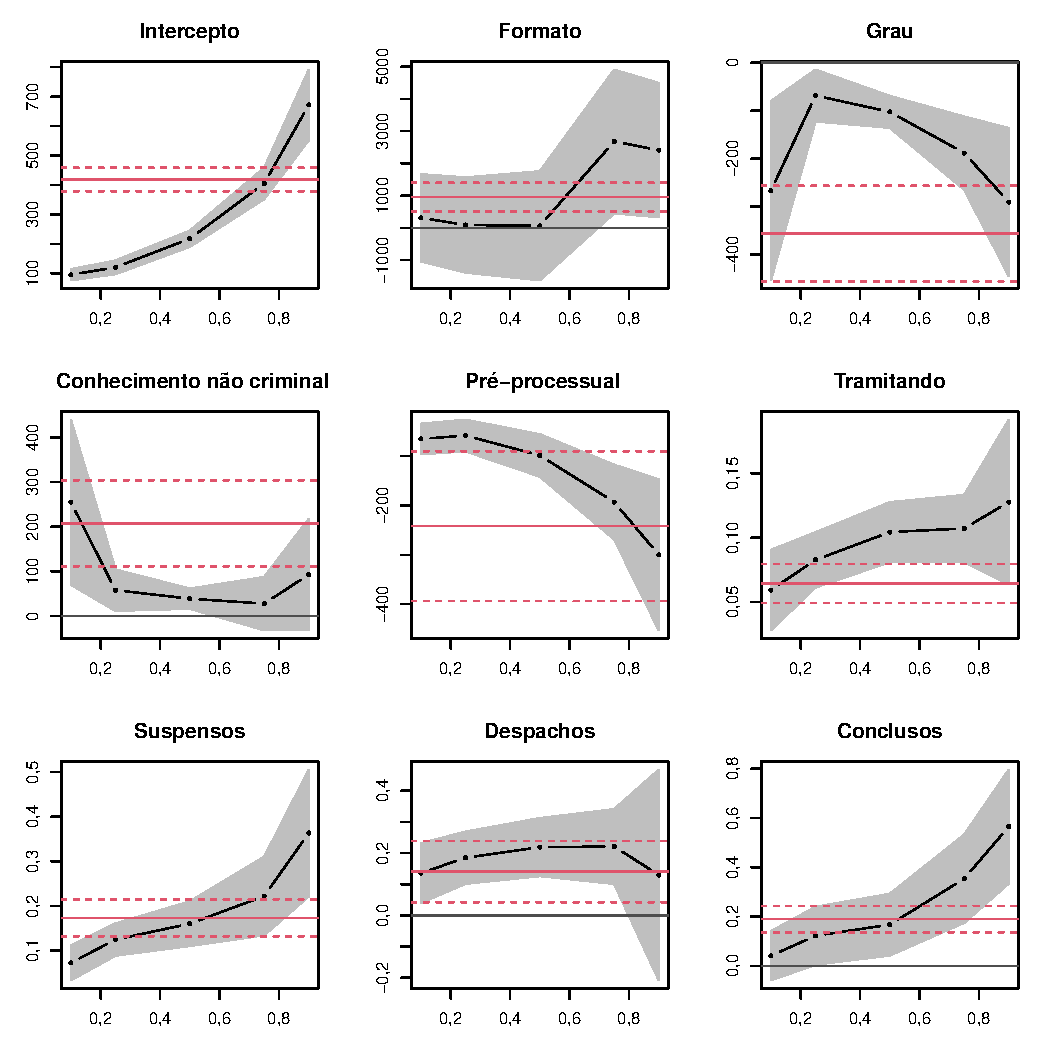
\includegraphics[scale=.9]{imagens/betas.pdf}    
    \label{fig:betas}
\end{figure}

Os coeficientes das variáveis quantitativas se mostraram diferentes em função do quantil ajustado, mostrando que a mudança dos hiperplanos não se trata de um mero deslocamento dos interceptos, mas de uma mudança da inclinação.

A linha sólida em vermelho representa o valor do coeficiente para o modelo linear ajustado com as mesmas covariáveis, e as linhas tracejadas representam os limites dos intervalos de confiança para o valor dos coeficientes. É notável que, no caso das variáveis "Suspensos" e "Conclusos", os coeficientes para a mediana e para o modelo linear são muito próximos, o que não ocorre com as outras covariáveis.

\subsubsection{Modelos de regressão gaussiana}
Para comparações posteriores com o modelo para a mediana, serão testados alguns modelos de regressão gaussiana. 

O Modelo \ref{tab:gr_selection} faz a seleção pelo stepwise através do menor AIC, seguida do stepwise do p-valor, considerando todas as covariáveis de forma linear, sem interações.

\begin{modelo}[H]
\centering
\caption{Regressão gaussiana} 
\label{tab:gr_selection}
\begin{tabular}{c|cc|c}
  \hline
\textbf{Variável} & \textbf{Coeficiente} & \textbf{Erro Padrão} & \textbf{P-valor} \\ 
  \hline
  Intercepto & 1,1 ano & 24 & \approx 0 \\ 
  Grau & -4,7 meses & 26 & \approx 0 \\ 
  Formato & 2,7 anos & 271 & \approx 0 \\ 
  Procedimento - Outros & -7,2 meses & 60 & \approx 0 \\ 
  Procedimento - Pré-processual & -8,8 meses & 91 & 0,003 \\ 
  Tramitando & 1h35min & 0,009 & \approx 0 \\ 
  Decisões & -9h43min & 0,06 & \approx 0 \\ 
  Conclusos & 4h32min & 0,033 & \approx 0 \\ 
  Suspensos & 4h10min & 0,025 & \approx 0 \\ 
  Despachos & 3h23min & 0,059 & 0,017 \\ 
  Audiências & 7 dias & 2 & 0,012 \\
   \hline
\end{tabular}
\end{modelo}

O modelo selecionado é muito parecido com o Modelo \ref{tab:candidate1_0,5}, com a adição das variáveis Formato e Audiências.

A variável Audiências não apareceu em nenhum dos modelos de regressão quantílica. No modelo gaussiano, por sua vez, ela apresentou o maior coeficiente entre as variáveis quantitativas, o que é esperado, dada a baixa amplitude da variável em relação às outras (Figura \ref{fig:cross_charts_without_outliers}).


O Modelo \ref{tab:gr_selection} apresenta o resultado da seleção de variáveis considerando as covariáveis presentes no Modelo 3, mais as interações entre elas e os termos quadráticos.

\begin{modelo}[H]
\centering
\caption{Regressão gaussiana com interações} 
\label{tab:gr_selection_interaction}
\begin{tabular}{c|cc|c}
  \hline
\textbf{Variável} & \textbf{Coeficiente} & \textbf{Erro Padrão} & \textbf{P-valor} \\ 
  \hline
  Intercepto & 1,3 ano & 21 & \approx 0 \\ 
  Grau & -7,4 meses & 23 & \approx 0 \\ 
  Procedimento - Pré-processual & -10,8 meses & 90 & \approx 0 \\ 
  Procedimento - Outros & -5,6 meses & 60 & 0,004 \\ 
  Formato & 2,5 anos & 268 & \approx 0 \\ 
  Tramitando & 2h18min & 0,012 & \approx 0 \\ 
  Decisões & -6h3min & 0,093 & 0,008 \\ 
  Despachos & -6h18min & 0,084 & 0,005 \\ 
  Conclusos & 3h10min & 0,039 & \approx 0 \\ 
  Rec. Interno Julgado$^{2}$ & 0h28min & 0,008 & 0,011 \\ 
  Suspensos:Despachos & 36 segundos & 6,8$\times10^{-5}$ & \approx 0 \\ 
  Despachos:Audiências & 1h39min & 0,013 & \approx 0 \\ 
  Suspensos:Conclusos & 36 segundos & 8,5$\times10{-5}$ & \approx 0 \\ 
  Suspensos:Audiências & -1h26min & 0,006 & \approx 0 \\ 
  Tramitando:Decisões & -5 segundos & 1,4$\times10^{-5}$ & \approx 0 \\
   \hline
\end{tabular}
\end{modelo}

Diferente dos modelos quantílicos, a seleção com transformações não-lineares escolheu uma transformação quadrática para a variável Recurso Interno Julgado, com coeficiente menor do que todas as variáveis sem transformações e interações. O resultado conta com cinco coeficientes estimados a mais do que o Modelo \ref{tab:candidate2_0,5}, que é o análogo para a mediana.

Muitas interações também foram consideradas significativas. Porém, como mostra o Modelo \ref{tab:gr_selection_interaction}, três delas apresentaram influência de poucos segundos, e tiveram o menor erro padrão entre os observados.

A Tabela \ref{tab:coefs_gauss} mostra os coeficientes presentes em cada um dos modelos gaussianos.

\begin{table}[H]
\centering
\caption{Coeficientes significativos para cada modelo gaussiano} 
\label{tab:coefs_gauss}
\begin{tabular}{c|cc}
  \hline
     \multirow{2}{*}{\textbf{Variável}} & \multicolumn{2}{c}{\textbf{Coeficiente}}   \\ \cline{2-3}
 & Modelo \ref{tab:gr_selection} & Modelo \ref{tab:gr_selection_interaction} \\ 
  \hline
  Intercepto & \checkmark & \checkmark \\
  Formato & \checkmark & \checkmark \\
  Procedimento - Pré-processual & \checkmark & \checkmark \\
  Procedimento - Outros & \checkmark & \checkmark \\
  Grau & \checkmark & \checkmark \\
  Tramitando & \checkmark & \checkmark \\
  Decisões & \checkmark & \checkmark \\
  Conclusos & \checkmark & \checkmark \\
  Despachos & \checkmark & \checkmark \\
  Suspensos & \checkmark &  \\ 
  Audiências & \checkmark &  \\ 
  Rec. Interno Julgado$^2$ &  & \checkmark \\ 
  Suspensos:Despachos &  & \checkmark \\ 
  Despachos:Audiências &  & \checkmark \\ 
  Suspensos:Conclusos &  & \checkmark \\ 
  Suspensos:Audiências &  & \checkmark \\ 
  Tramitando:Decisões &  & \checkmark \\
   \hline
\end{tabular}
\end{table}

A variável de "Recurso Interno Julgado" foi a única das variáveis do Modelo \ref{tab:gr_selection_interaction} que não apareceu de nenhuma forma no Modelo \ref{tab:gr_selection}, e só foi considerada significativa em uma transformação quadrática. As outras variáveis são todas comuns entre os modelos, embora não se apresentem na mesma configuração.

As variáveis Suspensos e Audiências, que estão presentes no Modelo \ref{tab:gr_selection} de forma independente, só são significativas no Modelo \ref{tab:gr_selection_interaction} com interações, tanto entre as duas, quanto com as outras variáveis independentes do modelo.

A Tabela \ref{tab:aic_bic_gaussianos} mostra o AIC e o BIC para cada modelo.

\begin{table}[H]
\centering
\caption{AIC, BIC, MAE e número de coeficientes para os modelos gaussianos} 
\label{tab:aic_bic_gaussianos}
\begin{tabular}{c|cccc}
  \hline
\textbf{Modelo} & \textbf{AIC} & \textbf{BIC} & \textbf{MAE} & \textbf{Coeficientes} \\ 
  \hline
Modelo \ref{tab:gr_selection} & 51.089 & 51.163 & 255 &  11 \\ 
  Modelo \ref{tab:gr_selection_interaction} & 51.023 & 51.121 & 252 &  15 \\  
   \hline
\end{tabular}
\end{table}

De forma análoga ao Modelo \ref{tab:candidate1_0,5} e ao Modelo \ref{tab:candidate2_0,5}, os modelos gaussianos sem transformações não são os que minimizam o AIC e o BIC. Os dois critérios consideram o Modelo \ref{tab:gr_selection_interaction} como o melhor, apesar de ter mais coeficientes estimados.

Apesar da superioridade no que se refere ao BIC e AIC, o Modelo \ref{tab:gr_selection_interaction} é muito menos interpretável que o Modelo \ref{tab:gr_selection}, característica que não é considerada pelo BIC e pelo AIC, e que será priorizada para os modelos de tendência central, tal qual como foi com as regressões para a mediana.

Enunciando o Modelo \ref{tab:gr_selection}, tem-se que uma audiência adicional aumenta o tempo médio até a baixa dos processos da vara em 7 dias, em média (mantendo as demais covariáveis constantes). O processo ser físico ao invés de eletrônico causa um aumento de mai de dois anos e meio no tempo, em média. Um processo em segundo grau, em média, leva cinco meses a menos para receber baixa do que um processo em primeiro grau. Quanto mais decisões o órgão julgador tomar, menor será o tempo médio até a baixa. Quanto maior o número de processos tramitando, maior é o tempo médio, mas um único processo a mais tramitando aumenta o tempo médio em quase duas horas, mantendo fixos os valores das outras covariáveis.

%Observando os erros médios absolutos nas tabelas \ref{tab:aic_bic_gaussianos} e \ref{tab:aic_tau0,5}, é notável que os modelos de regressão para a mediana performaram melhor do que os modelos gaussianos, mesmo que tenham utilizado de um número muito menor de coeficientes estimados. Isso vale tanto para os modelos com transformações quanto os modelos sem transformações, o que mostra que, além de informações sobre a distribuição das observações em torno do hiperplano, os modelos quantílicos também fornecem um bom desempenho preditivo.

